
\section{History I}

Circles rolling on circles are much more than a product of a novel toy. They have been used as a crucial tool in the understanding the universe around us.

It had been long believed in ancient times that the celestial bodies in the sky revolved around the Earth. This is known as the geocentric model of the universe. This seemed intuitively true, since the stars appear do appear to circle around the sky at night, and 

However, the geocentric model could not explain one certain behaviour, that being the movement of the planets. The word ''planet`` comes from the Greek word ``planetai'', meaning ``wandering star''. Even with the naked eye, it can be observed that the planets do not move in a well-ordered way. They would slow down, speed up, and sometimes move backward. This strange behaviour of the planets is referred to as \textit{retrograde motion}).
 \begin{figure}[H]
     \centering
     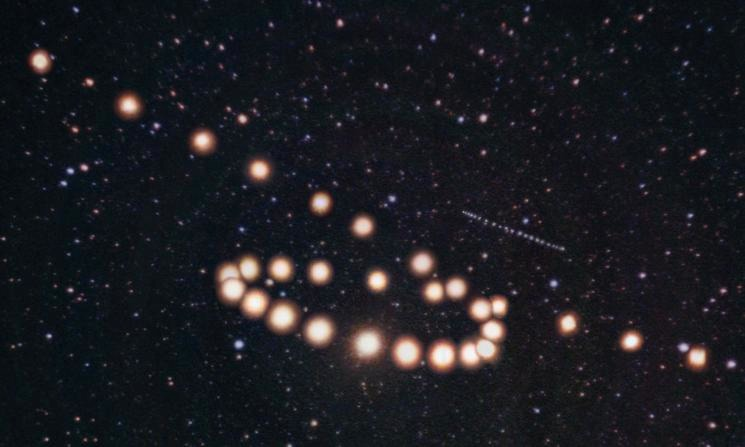
\includegraphics[width=0.75\textwidth]{figures/marsRetro.jpg}
     \caption{The retrograde motion of Mars making a "loop" across the sky over several weeks.}
     \label{fig:my_label}
 \end{figure}

I plotted the daily positions of Mars and Venus from September 1987 to November 2019 relative to Earth (geocentric) using data from JPL HORIZONS, an online ephemeris.  

\begin{figure}[H]%
    \centering
    \subfloat[Geocentric Venus]{{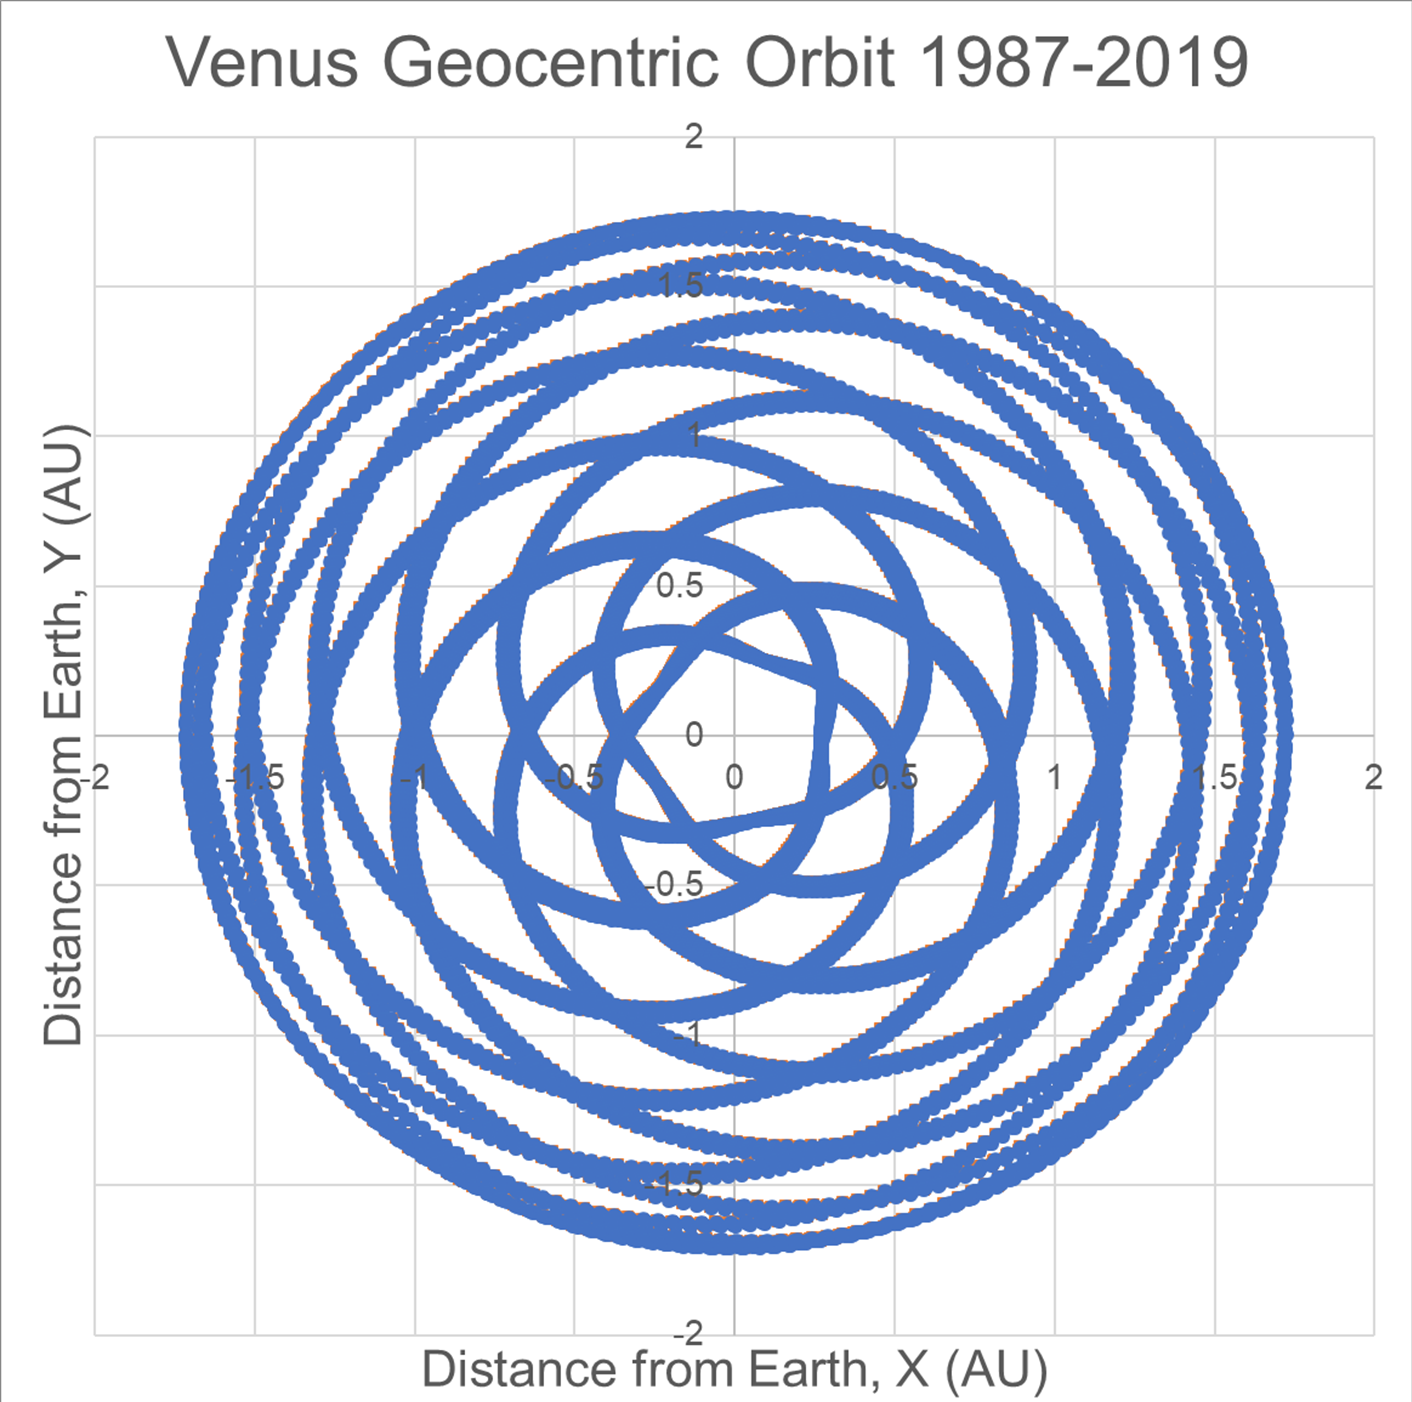
\includegraphics[width=0.46\textwidth]{figures/venus.png} }}%
    \qquad
    \subfloat[Geocentric Mars]{{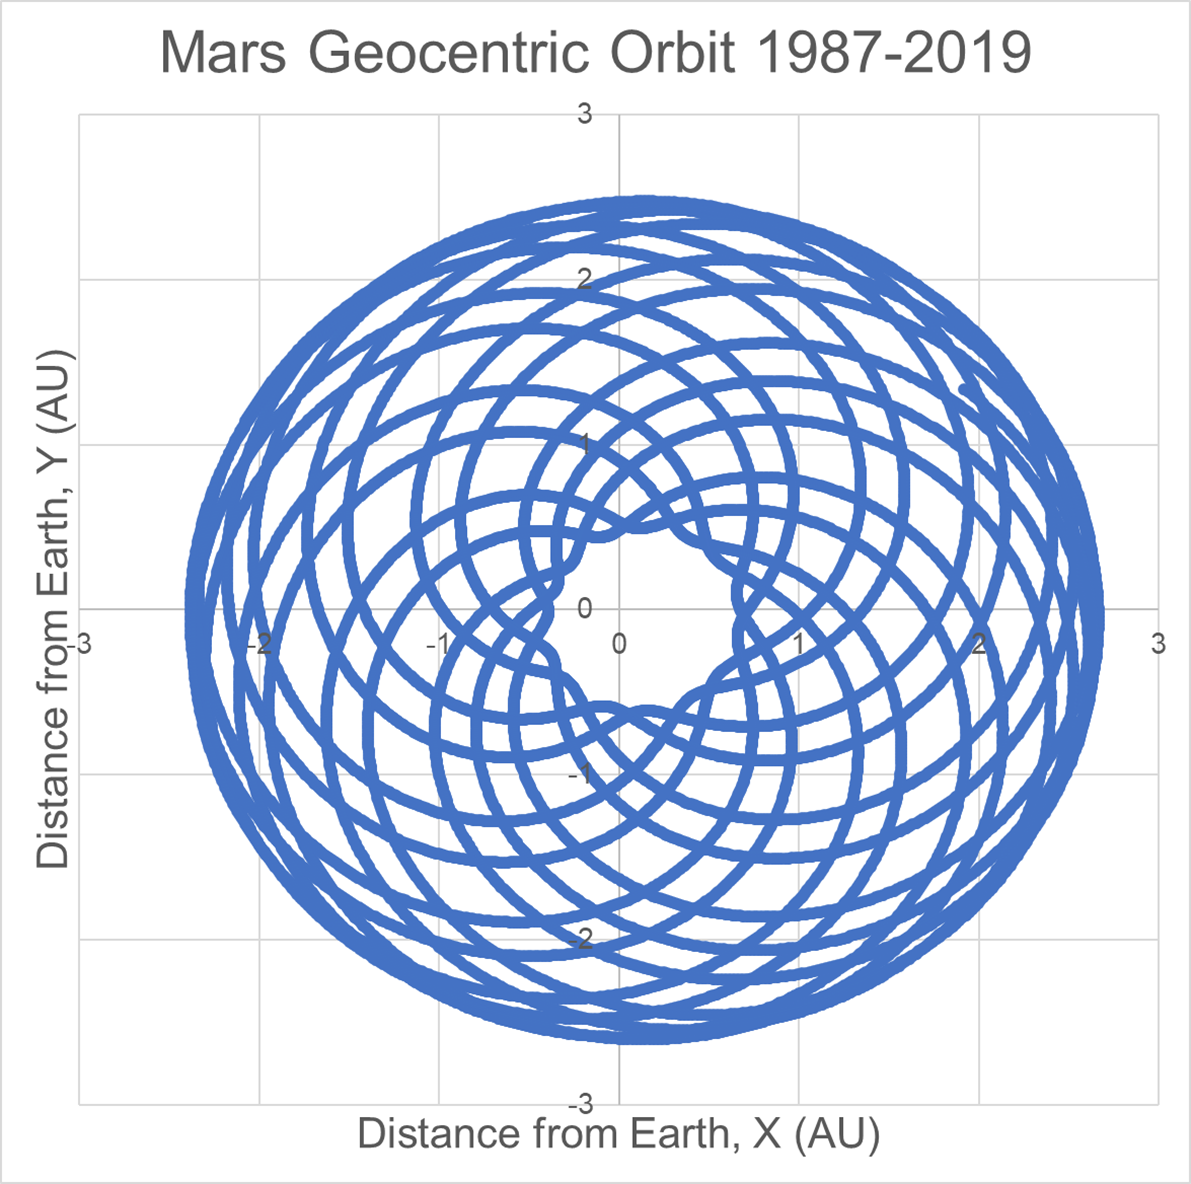
\includegraphics[width=0.46\textwidth]{figures/mars.png} }}%
    \caption{Geocentric orbits of Venus and Mars.}%
    \label{fig:example}%
\end{figure}

Around 2nd century AD, Ptolemy proposed his model of the solar system, refining upon the geocentric model of the Greeks (that is, the belief that all celestial bodies revolved around the Earth). 



Ptolemy proposed his model which solved this problem of retrograde motion. His model made use of what he called \textit{epicycles} and \textit{deferents}. 

Here are the parametric equations of a simple deferent and epicycle system:
\begin{centering}
$y(t) = (R+r)sin(at) + rsin(bt)$ \\ 
$x(t) = (R+r)cos(at) + rcos(bt)$ \\
\end{centering}

Notice that these sets of equations are very similar to the epicycloid equations, except that the sines and cosines are being added up, and the frequency (or turning speed) of each circle is variable. We can consider this as a more generalized version of our epicycloid. 



\begin{figure}[h]
    \centering
    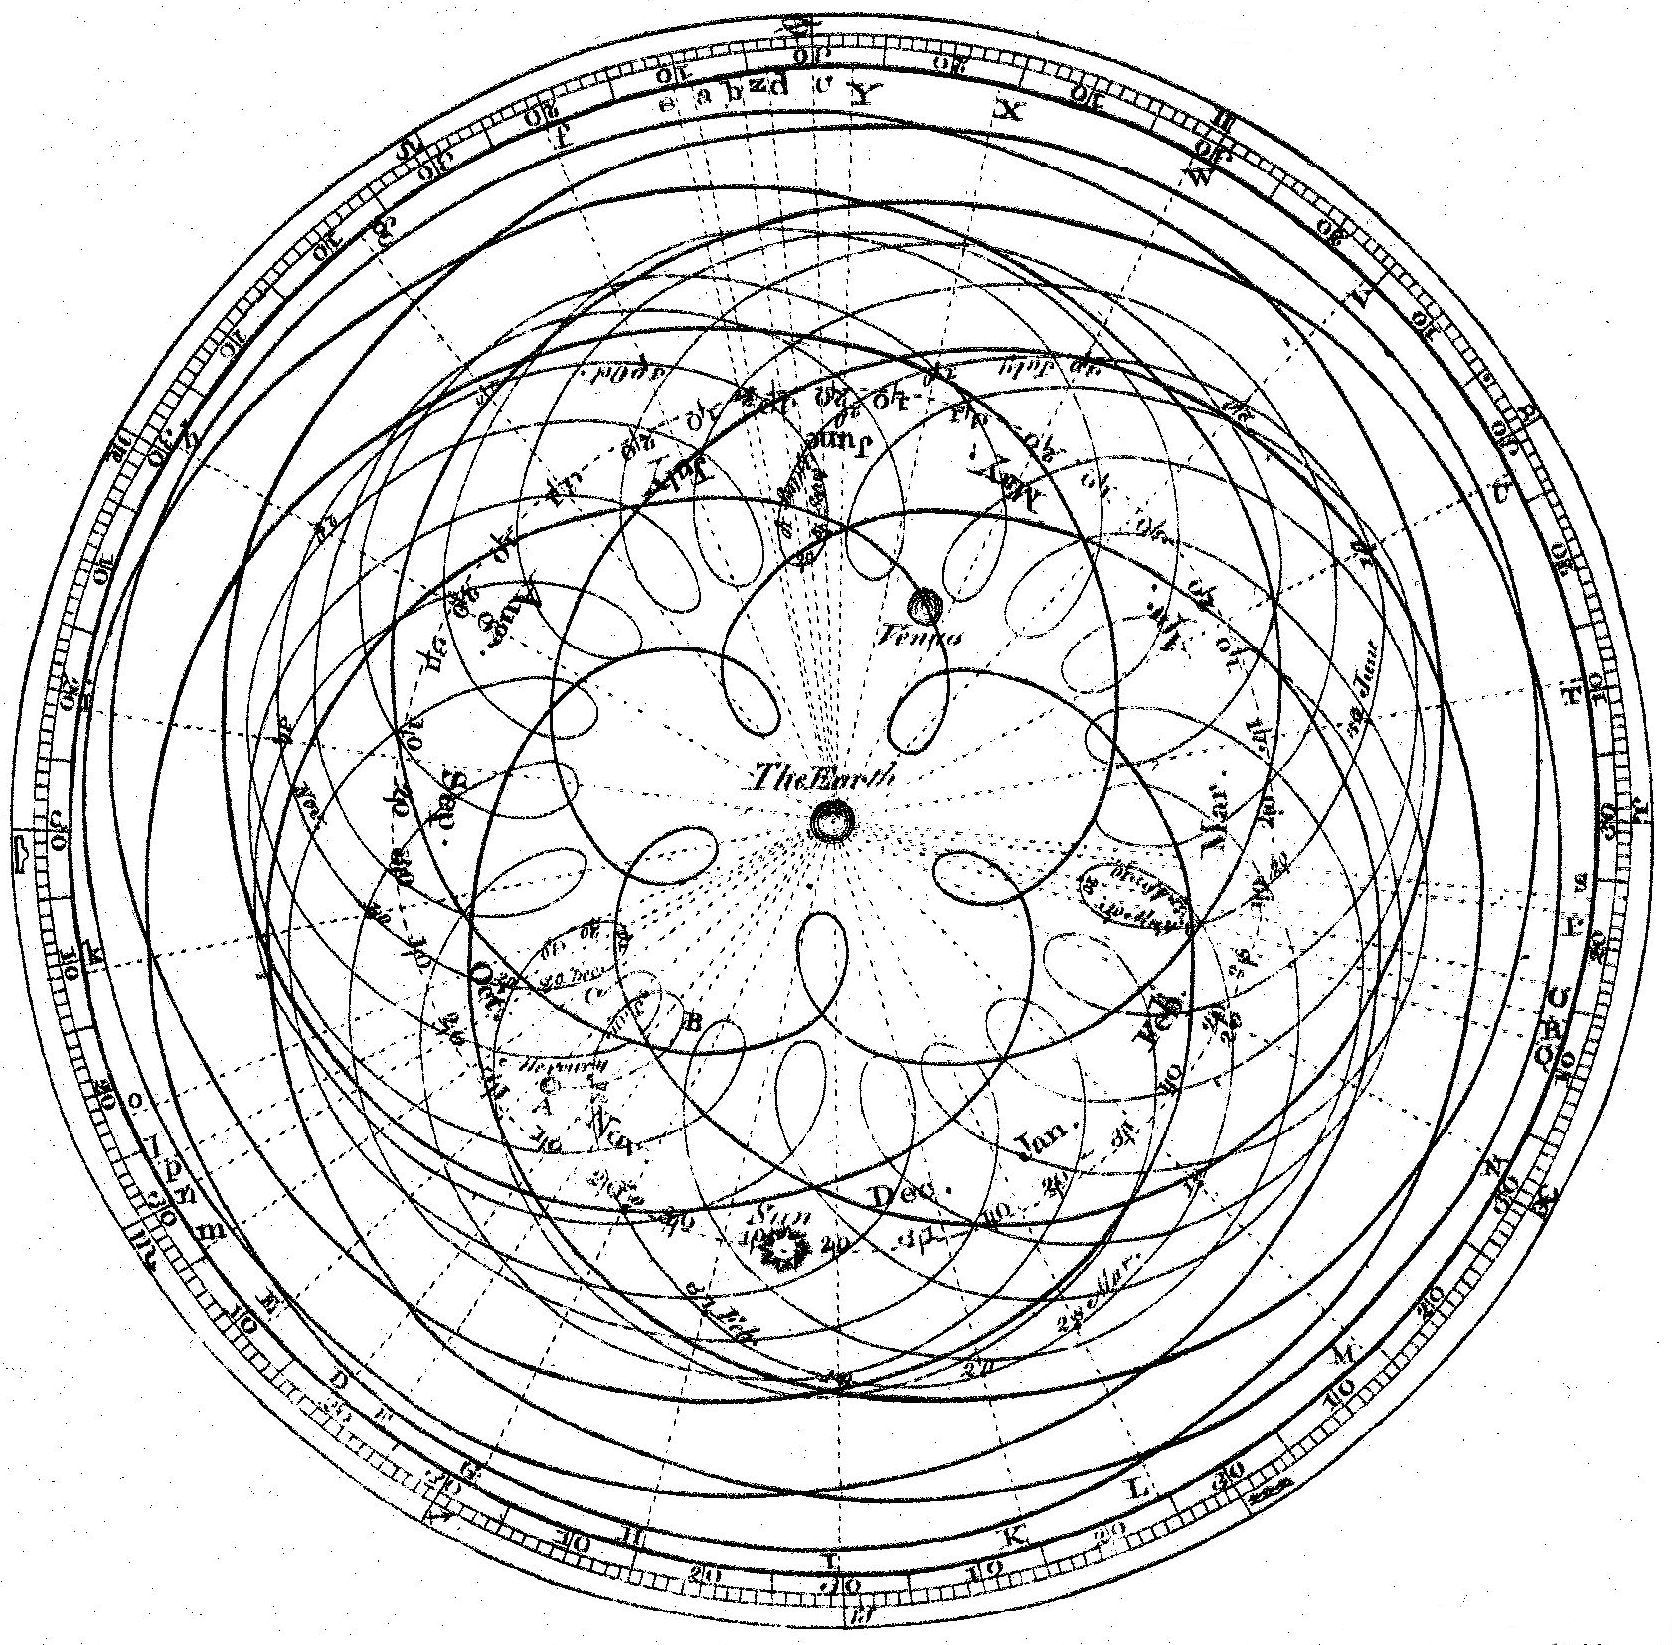
\includegraphics[width=9cm]{figures/ptolemaic_model.jpg}
    \caption{A 1777 Encyclopædia Britannica illustration of the paths traced by planets according to the epicycle geocentric model.}
    \label{fig:my_label}
\end{figure}
\section{History II}

Belief in Ptolemy’s geocentric model lasted until the 16th century - an astonishing 1400 years! It is now known that the geocentric model is false


It is commonly taught that one reason why the Ptolemy's deferent-epicycle fell out of fashion was due to the addition of more and more epicycles in an attempt to increase the accuracy of the model in fitting the observed data. A 2002 astronomy lecture at UC Berkeley claimed (citing no sources) that at ``one point the geocentric model had as many as 80 epicycles within epicycles'' http://cse.ssl.berkeley.edu/bmendez/ay10/2002/notes/lec6.html. The term ``adding epicycles'' or ``epicyclic'' became used to describe incorrect theories that fit the observed data but are unnecessarily complex and could be explained just as well with a much simpler theory. However, there is no historical evidence to back up the claim that Ptolemy or other supporters of the geocentric model used nearly as many epicycles as it is often said to contain. Typically, only one epicycle and deferent was used per planet. Copernicus's motive for introducing the heliocentric model came not from any excess use of epicycles to describe geocentricism. Instead, he felt that Ptolemy's model was “neither sufficiently absolute nor sufficiently pleasing to the mind” because “certain equants had to be conceived”. The equant was a highly controversial concept that Ptolemy employed which essentially shifted the Earth slightly away from the center of the deferent in order to increase model accuracy. Exploring the equant is out of the scope of this essay.
